\documentclass{article}
\usepackage[english]{babel}
\usepackage[letterpaper,top=2cm,bottom=2cm,left=3cm,right=3cm,marginparwidth=1.75cm]{geometry}
\usepackage{amsmath}
\usepackage{amssymb}
\usepackage{graphicx}
\usepackage[colorlinks=true, allcolors=blue]{hyperref}
\usepackage{polski}
\usepackage{enumitem}
\newcommand{\probP}{\text{I\kern-0.15em P}}

\title{Data mining - zadanie 2}
\author{Gabriel Budziński}

\begin{document}
\maketitle

\section{Treść}
Recall what is the bias and variance of an estimator. Give examples of biased and unbiased
estimators.

\section{Rozwiązanie}

\begin{itemize}
    \item Bias - odległość wartości oczekiwanej estymatora od wartości parametru
    \item Variance - Odchylenia wartości estymatora od wartości oczekiwanej (po prostu jego wariancja)
\end{itemize}

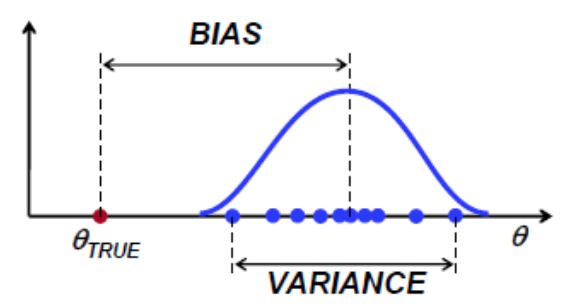
\includegraphics[scale=0.5]{b&v.png}
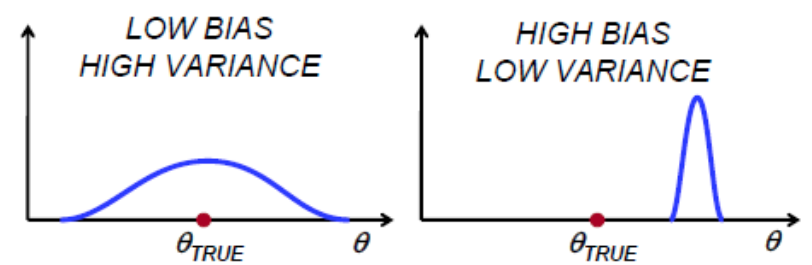
\includegraphics[scale=0.5]{b&v_tradeoff.png}
\\
\begin{itemize}
    \item Bias estymatora $\bar{\theta}$ parametru $\theta$ zdefiniowany jest jako $bias(\bar{\theta}) = E[\bar{\theta}] - \theta$
    \item Estymator jest nieobciążony kiedy $bias(\bar{\theta}) = 0$, czyli $E[\bar{\theta}] = \theta$
\end{itemize}

\subsection*{Przykład estymatora nieobciążonego}

Weźmy zmienne losowe $X_1,X_2,\dots,X_n$ i zaproponujmy estymator wartości oczekiwanej $\mu$:

\[\bar{\mu} = \frac{1}{n}\sum_{i=1}^{n}{X_i}\]

Znajdźmy $E[\bar{\mu}]$:

\[E[\bar{\mu}] = E\left[\frac{1}{n}\sum_{i=1}^{n}{X_i}\right] = \frac{1}{n}\sum_{i=1}^{n}{E[X_i]} = \frac{1}{n}\sum_{i=1}^{n}{\mu} = \frac{1}{n}n\mu = \mu\]

Skoro $E[\bar{\mu}] = \mu$, to $\bar{\mu}$ jest estymatorem nieobciążonym.

\subsection*{Przykład estymatora obciążonego}

Zaproponujmy estymator wiaruancji zmiennych losowych, gdzie $\bar{\mu}$ jest nieobciążonym estymatorem wartości oczekiwanej.

\[\bar{\sigma}^2 = \frac{1}{n}\sum_{i=1}^{n}{{(X_i - \bar{\mu})}^2} = \frac{1}{n}\sum_{i=1}^{n}{(X_i^2 - 2X_i\bar{\mu} + \bar{\mu}^2)} = \frac{1}{n}\sum_{i=1}^{n}{X_i^2} - 2\bar{\mu}\overbrace{\frac{1}{n}\sum_{i=1}^{n}{X_i}}^{\text{$\bar{\mu}$}} + \frac{1}{n}n\bar{\mu}^2 = \frac{1}{n}\sum_{i=1}^{n}{X_i} - \bar{\mu}^2\]

Z tego dalej

\[E[\bar{\sigma}^2] = E\left[\frac{1}{n}\sum_{i=1}^{n}{X_i} - \bar{\mu}^2\right] = \frac{1}{n}\sum_{i=1}^{n}{E[X_i]} - E[\bar{\mu}^2] = \frac{1}{n}\sum_{i=1}^{n}{(\sigma^2 + \mu^2)} - \left(\frac{\sigma^2}{n} + \mu^2\right) = \sigma^2 + \mu^2 - \frac{\sigma^2}{n} - \mu^2 = \frac{(n-1)\sigma^2}{n}\]

Jak łatwo zauważyć, ten estymator ma bias $\frac{n-1}{n}$. Aby się go pozbyć, wystarczy przemnożyć go przez $\frac{n}{n-1}$



\end{document}